\begin{center}
    {\LARGE \textbf{2013有机化学}} \\[2ex]
    {\large 时量180分钟 \quad 满分150分}
\end{center}

\vspace{0.5cm}
\noindent\textbf{注意事项:}
\begin{enumerate}[label=\arabic*., parsep=0pt, itemsep=0pt]
    \item 答题前,考生先将自己的姓名、学号、考场号、座位号填写在答题卡上,将条形码准确粘贴在考生信息条形码粘贴区。
    \item 考试结束后,将本试卷与答题纸一并收回。
    \item 回答各个问题时,将答案写在答题纸上,写在本试卷上无效。
\end{enumerate}

\vspace{0.5cm}
\noindent\textbf{一、完成反应(30 pts.)}

\begin{enumerate}[label=\arabic*., itemsep=3ex]
    \item 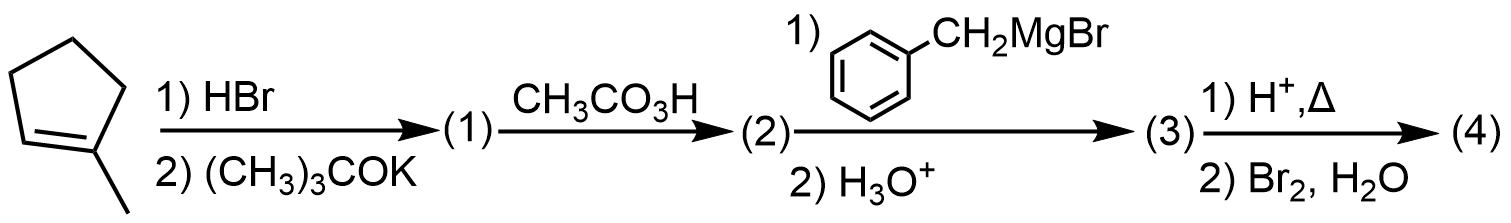
\includegraphics[scale=0.3, valign=c]{./Figure/2013/2013_1_1.png} 
    \item 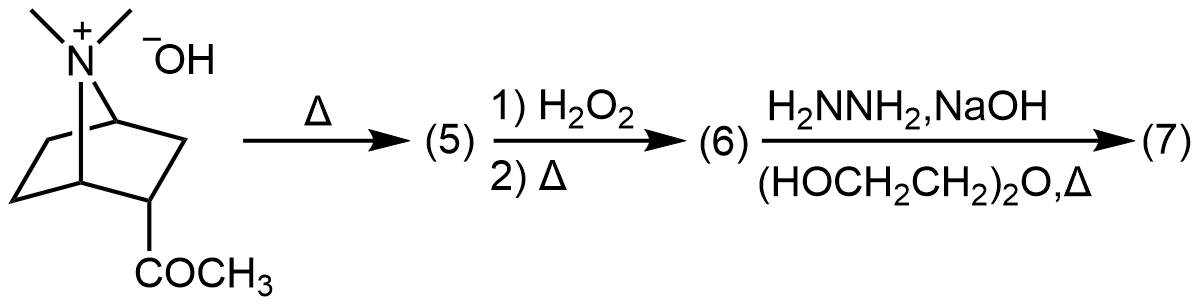
\includegraphics[scale=0.3, valign=c]{./Figure/2013/2013_1_2.png}
    \item 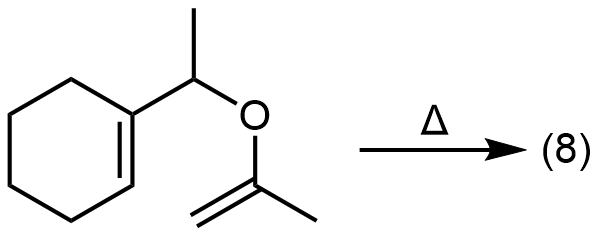
\includegraphics[scale=0.3, valign=c]{./Figure/2013/2013_1_3.png}
    \item 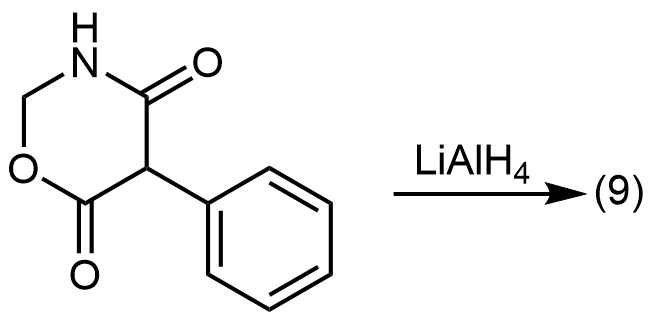
\includegraphics[scale=0.3, valign=c]{./Figure/2013/2013_1_4.png}
    \item 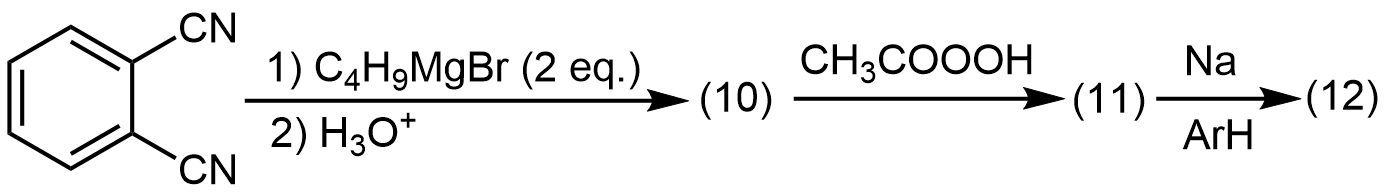
\includegraphics[scale=0.3, valign=c]{./Figure/2013/2013_1_5.png}
    \item 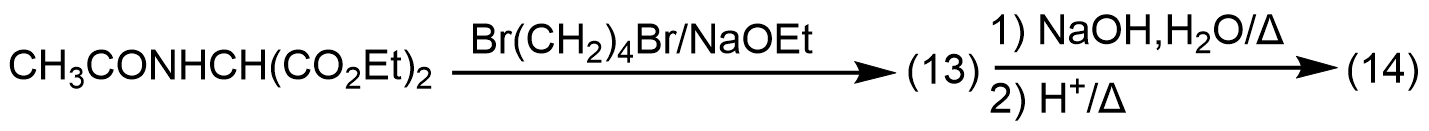
\includegraphics[scale=0.3, valign=c]{./Figure/2013/2013_1_6.png}
    \item 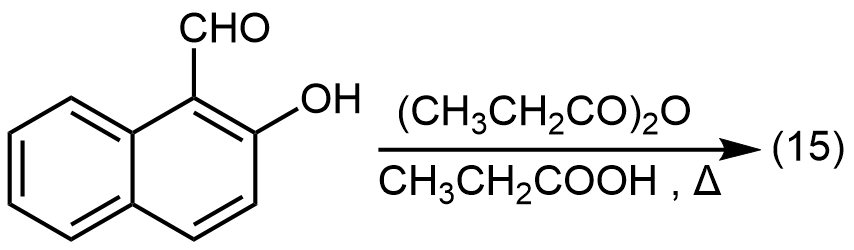
\includegraphics[scale=0.3, valign=c]{./Figure/2013/2013_1_7.png}

\end{enumerate}

\vspace{0.5cm}
\noindent\textbf{二、机理题(30 pts.)}

\begin{enumerate}[label=\arabic*., start=1, itemsep=1.5ex]
    \item 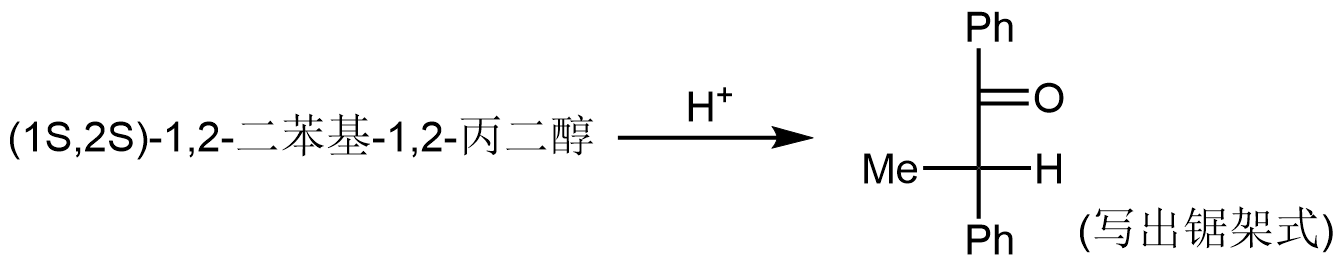
\includegraphics[scale=0.3, valign=c]{./Figure/2013/2013_2_1.png}
    \item 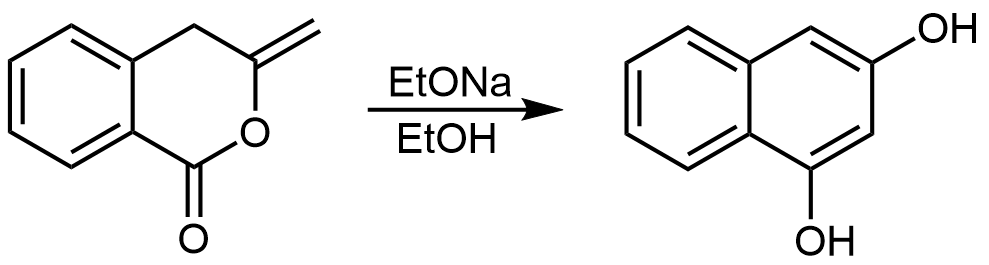
\includegraphics[scale=0.3, valign=c]{./Figure/2013/2013_2_2.png}
    \item 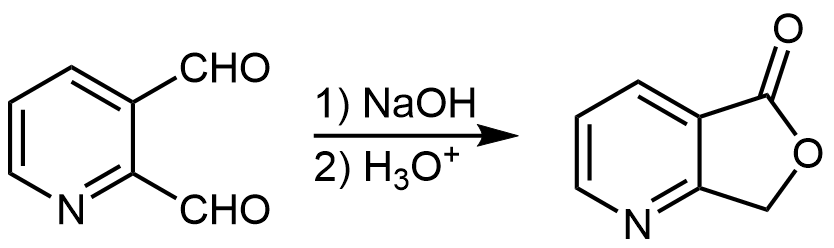
\includegraphics[scale=0.3, valign=c]{./Figure/2013/2013_2_3.png}
\end{enumerate}

\vspace{0.5cm}
\noindent\textbf{三、合成题(30 pts.)}

\begin{enumerate}[label=\arabic*., start=1, itemsep=1.5ex]

    \begin{figure}[htbp]
        \centering
        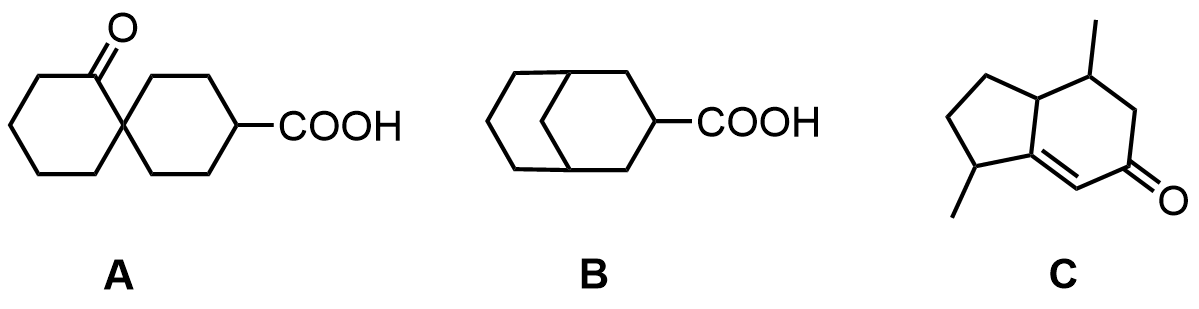
\includegraphics[scale=0.3]{./Figure/2013/2013_3.png}
    \end{figure}
    \item 以双环[4,4,0]癸烷和乙烯为原料合成\textbf{A}
    \item 以小于等于3个碳的有机物为原料合成\textbf{B}
    \item 以小于等于3个碳的有机物为原料合成\textbf{C}
\end{enumerate}

\vspace{0.5cm}
\noindent\textbf{四、综合题(30 pts.)}

\begin{center}
    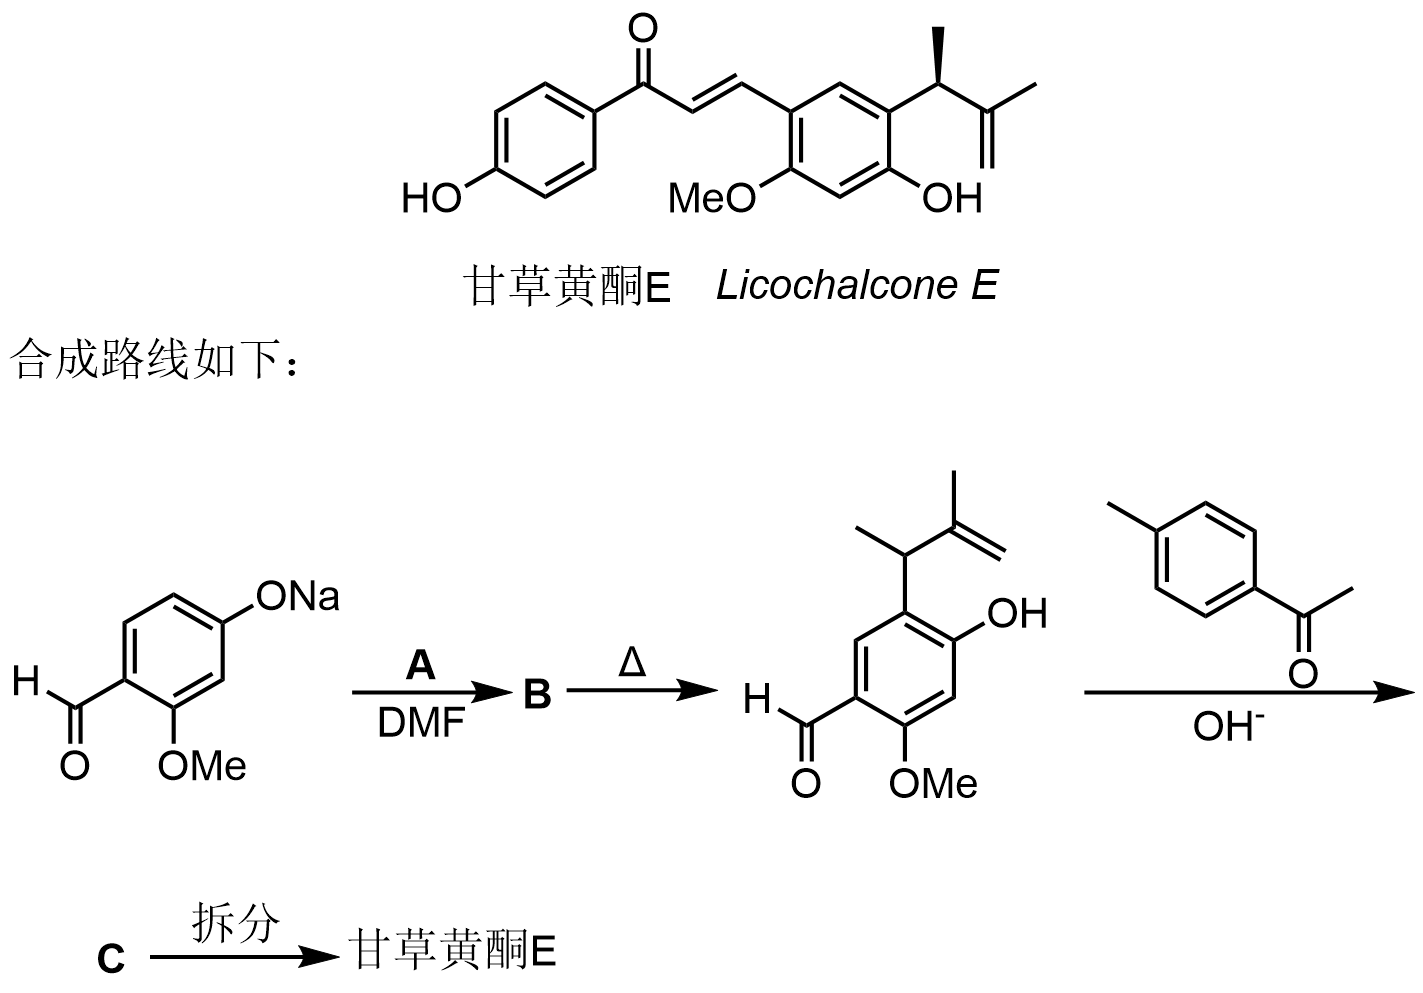
\includegraphics[scale=0.3]{./Figure/2013/2013_4.png}
\end{center}

\begin{enumerate}[label=\arabic*., itemsep=1.2ex]
    \item 请写出化合物A、B和C的结构式。(6 pts.)
    \item 请写出甘草黄酮E中手性碳原子的绝对构型。(2 pts.)
    \item 某同学拆分得到旋光度值为“+”，ee值为90\%的甘草黄酮E，请计算产品中比旋光度为“+”的异构体的含量。(2 pts.)
    \item 请写出化合物2生成化合物C的反应机理。(6 pts.)
    \item 以小于等于3个碳的有机物为原料及必要的试剂，采用最简短的步骤合成A。(6 pts.)
    \item 以苯及小于等于3个碳的有机物为原料及必要的试剂合成2-甲氧基-4-羟基苯甲醛。(8 pts.)
\end{enumerate}

\vspace{0.5cm}
\noindent\textbf{五、实验题 略}